\section{Scaling our Approach to any Boolean Circuit}
\label{sec:p_encodings_graphs}

Our framework optimizes the homomorphic evaluation of single Boolean functions but suffers the following limitations:

\begin{enumerate}
    \item For a Boolean function with a high number of inputs, the search algorithm may be very time-consuming.
    \item Some functions simply do not have any solution for acceptable values for $p$ ($p < 32$ for example) and thus are not efficiently evaluable in a single \gls{PBS}.\footnote{The \gls{PBS} can be evaluated for larger values of $p$ but it quickly becomes inefficient as $p$ grows.}
\end{enumerate}


As a consequence, we need a solution to extend our framework to these cases. In this section, we propose a strategy to leverage the circuit representation of a ``tough'' function $f$ to find a strategy of homomorphic evaluation with as few bootstrappings as possible.


\subsection{Graph of Subcircuits}
\label{sec:graph_definition}

Let $f: \B^\ell \longrightarrow \B$ be a Boolean function, and let $\mathcal{F}$ be a Boolean circuit representing $f$ (some preliminaries about Boolean circuits can be found in Section \ref{sec:p_encodings_preliminaries_boolean}). Let us describe the layout of the circuit $\mathcal{F}$. It has $\ell$ input wires, denoted by $\{y_j\}_{1 \le j \le \ell}$, and the output wire is denoted by $z$. The intermediary wires are denoted by $\{t_j\}_{1 \le j \le \theta}$. The Boolean operation gates are of fan-out 1. 


Our goal is to split the circuit into a directed acyclic graph $\mathcal{G}$, whose vertexes are subcircuits $\{\mathcal{F}_1, \dots, \mathcal{F}_k\}$ and whose edges connect the outputs of a subcircuit with the input of another. Each subcircuit $\mathcal{F}_i$ represents a subfunction $f_i: \B^{l_i} \mapsto \B$ that is evaluable with a gadget with our framework. 

We use the same notations to refer to the elements of a subcircuit $\mathcal{F}_i$ and we index them with $i$. The output of $\mathcal{F}_i$ is denoted by $z^{(i)}$ and its inputs by $\{y_j^{(i)}\}_{1 \le j \le \ell}$ and so on. 


The graph is valid for $f$ with respect to modulus $p$ if the following properties are satisfied:
\begin{itemize}
    \item Each subcircuit $\mathcal{F}_i$ has only one output $z^{(i)}$.
    \item For a subcircuit $\mathcal{F}_i$, all its inputs are either inputs of the whole circuit or outputs of other subcircuits of the graph. We can write this property as:
    $$
    \{y_j^{(i)}\}_{1 \le j \le l_i} \subset \left ( \{y_j\}_{1 \le j \le \ell} \cup \{z^{(j)}\}_{1 \le j < i} \right )
    $$
    Thus, the indexing of the $\mathcal{F}_i$'s respects the topological order of the graph, i.e. no gates of $\mathcal{F}_i$ has a child in any of the $\mathcal{F}_j$, with $j < i$.
    \item All the Boolean functions $f_i$ represented by the subcircuits $\mathcal{F}_i$ are evaluable in a single bootstrapping with modulus $p$ with our proposed method. 
    \item The last subcircuit $\mathcal{F}_c$ of the graph has $z$ (the output of the main circuit) for output: $z^{(c)} = z$.
\end{itemize}

\begin{figure}
    \centering
    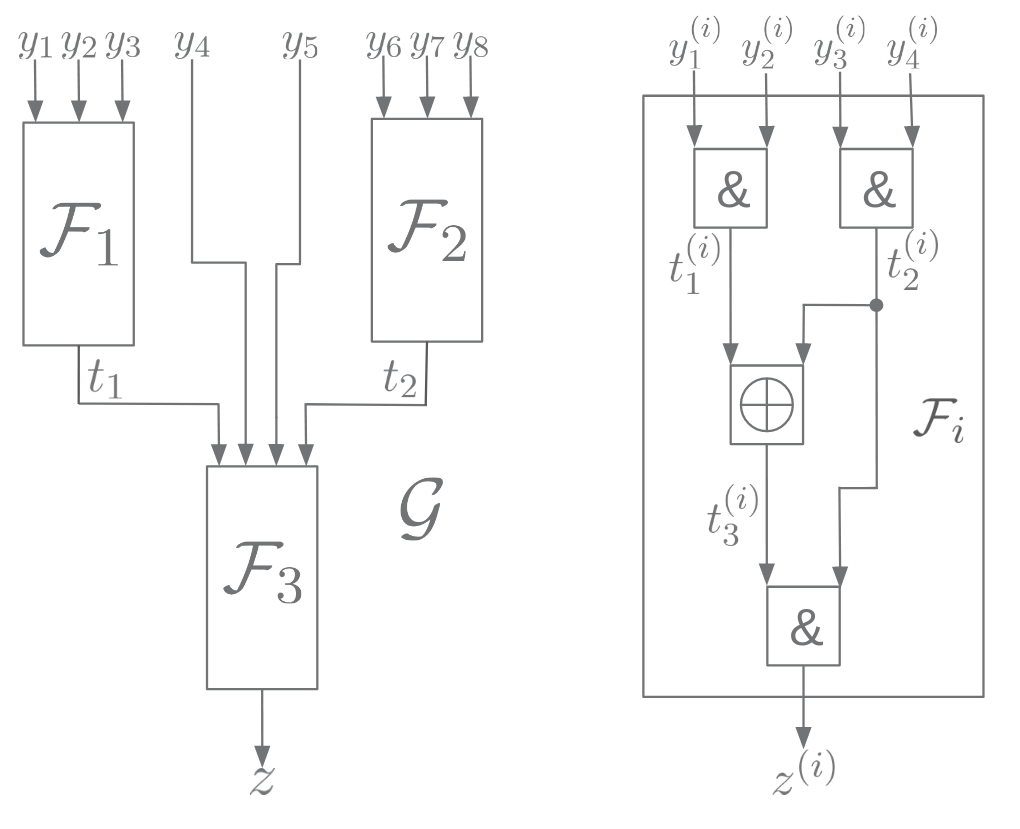
\includegraphics[width=0.75\textwidth]{img/to_harmonize/graphs.png}
    \caption{Example of graph of subcircuits (on left) and of a valid subcircuit (on right). Each subcircuit $\mathcal{F}_i$ is evaluated homomorphically with a gadget $\Gamma_i$.}
    \label{fig:enter-label}
\end{figure}




To homomorphically evaluate the function $f$, we evaluate each subcircuits with one bootstrapping for each of them and get the final result. In order to reduce the cost of evaluation for a given $p$, the goal is hence to find the \emph{smallest} valid graph possible in terms of number of subcircuits. Taking a greater value of $p$ produces a different graph that may be smaller (as subcircuits might be larger), but the timings of bootstrapping in this graph might on the other hand be greater. One can therefore run the search for different values of $p$ and keep the most efficient setup among the possible graphs. %Additionally, for some values of $p$, such a graph may not exist.

\subsection{Heuristics to Find a Small Graph}
\label{sec:heuristics_graph}

Finding such a graph can be done by exhaustively evaluating all the possible subcircuits with our method introduced in Section \ref{sec:p_encodings_search}, and then find the more efficient one. However it is not really practical to evaluate \emph{all} the possible subcircuits, so we develop some heuristics to reduce the search space. Let us start by defining a few bounds on the considered subcircuits, we will leave the other ones apart in our algorithm:

\begin{itemize}
    \item The subcircuits have at most $B$ inputs ($\forall i, l^{(i)} < B$). The purpose of this bound is to limit the running time of Algorithm \ref{alg:add_element}. In practice, for our experiments, we took $B = 10$.
    \item The subcircuits are evaluable with one single bootstrapping with a maximum value $p_{max}$. This value ensures a bootstrapping with a reasonable timing. If the search algorithm fails for $p_{max}$, the subcircuit is dropped without trying to extend $p$. In our experiment, we took $p_{max}=31$.
\end{itemize}


In order to decompose our Boolean circuit into a graph satisfying the above property for a modulus $p$, we would want to exhaustively search all the subcircuits of $\mathcal{F}$ compliant with the bounds we introduced earlier. However, all subcircuits are not equally worth to evaluate. In particular a wire incoming a copy gate is particularly worth evaluating because is costs one bootstrapping but produce several inputs for the next subcircuits. 

We gather wires that precede a copy gate in the set $\mathcal{Z}$. We add to this set the global output $z$. We also gather the input wires of the global circuit $\mathcal{F}$ in the set $\mathcal{Y}$. We define the notion of \textit{atomic subcircuit} that is a valid subcircuit whose all inputs belong to $\mathcal{Y} \cup \mathcal{Z}$ and whose output belongs to $\mathcal{Z}$. Note that the merge of two atomic subcircuits that respect the global circuit wiring is also an atomic subcircuit.

\medskip

Our heuristic works as follows:

\begin{enumerate}
    \item For each of these outputs $z_i \in \mathcal{Z}$, we exhaustively construct a set $\widehat{\mathcal{F}_{z_{i}}}$ that gathers all the atomic subcircuits whose output is $z_i$.
    We then filter out the subcircuits of $\widehat{\mathcal{F}_{z_{i}}}$ that do not comply with the bounds introduced at the beginning of the section or that are not evaluable with a gadget with the input modulus $p$ (we use Algorithm \ref{alg:add_element} to decide that).
    \medskip
    \item Now we want to construct the smallest valid graph evaluating $\mathcal{F}$ using subcircuits from the $\widehat{\mathcal{F}_{z_{i}}}$'s. While finding the smallest graph is hard, constructing any valid graph is easy. As a consequence, our strategy to find a small graph is to randomly create a lot of valid graphs and to take the smallest one. The procedure to create a valid graph is the following: we start from the output $z$ and we randomly draw a subcircuit $\mathcal{F}_z$ from $\widehat{\mathcal{F}_z}$. The inputs of $\mathcal{F}_z$ can be sorted into two categories: the ones belonging to $\mathcal{Y}$ and the ones belonging to $\mathcal{Z}$. For each one of these latter wires $w \in \mathcal{Z}$, we repeat the procedure, i.e. we draw a subcircuit $\mathcal{F}_w$ from $\widehat{\mathcal{F}_w}$, and so on. When we have reached all the input wires of $\mathcal{F}$, we get a valid graph $\mathcal{G}$ . This second step is run a large amount of times (the number of trials is a parameter of the method), and the smallest graph, i.e. the one with the fewest subcircuits, is returned.
\end{enumerate}

We carried on this method on the S-box of \gls{AES} in Section \ref{sec:p_encodings_aes}.

\subsection{Parallelization of the Execution of the Graph}
\label{sec:parallelization}

Once we have our graph $\mathcal{G}$, we can identify its $n_\mathcal{L}$ \emph{layers}. Formally, they are defined as:

\begin{definition}
    A layer $\mathcal{L}$ of a graph $\mathcal{G}$ is a set of subcircuit $\{\mathcal {F}_\alpha, \dots, \mathcal{F}_\omega\}$ of $\mathcal{G}$ that verifies: $\forall \mathcal{F}_i, \mathcal{F}_j \in \mathcal{L}, \mathcal{F}_i \text{ is not an ancestor node of } \mathcal{F}_j.$    
\end{definition}

By construction, all the subcircuits belonging to the same layer can be evaluated in parallel. This reduces the number of bootstrapping steps from $k$ (the number of subcircuits in the graph $\mathcal{G}$) to $n_\mathcal{L}$ (the number of layers). Our graph-finding heuristic can be tweaked to select the graph with minimum number of layers instead of minimum number of subcircuits to optimize parallelization.
